% code to pdf: ctrl + alt + j
\chapter{System Model}
\label{chap:model}
% system flow diagram
% satellite orbit pattern
\section{System Overview}

This chapter introduces the LEO satellite communication system, as illustrated in Figure~\ref{fig_system}. We consider one of the satellites in the LEO satellite communication system. It consists of $M$ beams, represented by $\mathcal{M} = \{m\ |\ m = 1, 2, \ldots, M\}$. In the coerage area of the satellite, it contains $K$ cells, indexed by $\mathcal{K} = \{k\ |\ k = 1, 2, \ldots, K\}$. To achieve optimal coverage and minimize overlap, all ground cells are arranged in a regular hexagonal grid, ensuring uniform cell size. There are $U$ user equipments (UEs) in the coverage area, indexed by $\mathcal{U} = \{u\ |\ u = 1, 2, \ldots, U\}$. 

\begin{figure}[h!]
    \centering
    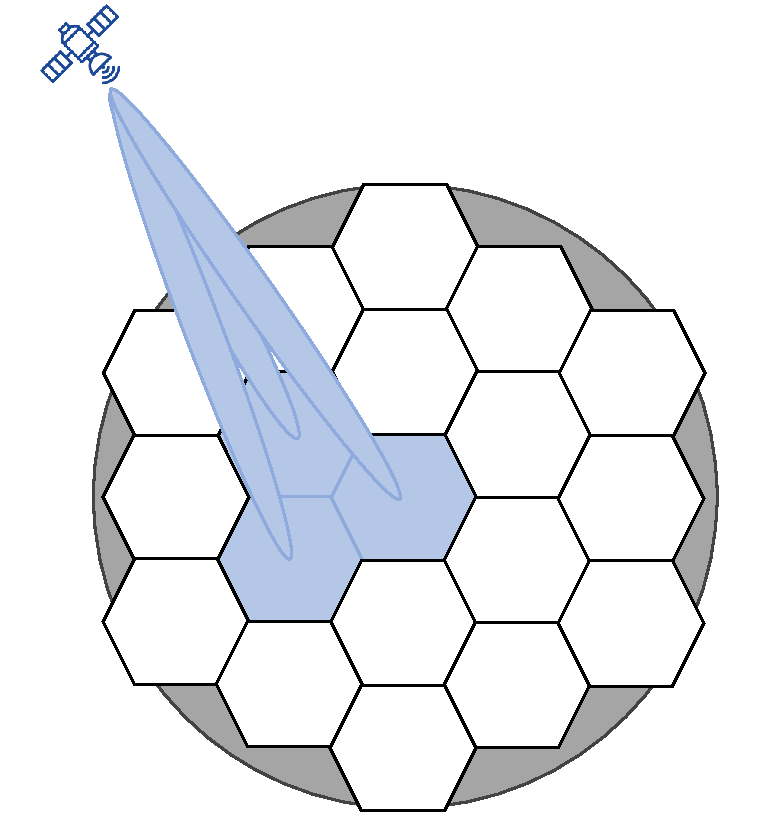
\includegraphics[width=0.8\textwidth]{figure/system overview2.pdf}
    \caption{Illustration of satellite beams and cells.}
    \label{fig_system}
\end{figure}
% TODO: time slot definition
We define a short time $T^{slot}$ as the time duration of a time slot, and $T^{total}$ as the total time that the satellite serves the area. Thus, there are $T^{total} / T^{slot}$ time slots in total service time, denoted as $\mathcal{T} = \{t\ |\ t = 1, 2, \ldots, T^{total} / T^{slot}\}$.

In this thesis, we adopt the quasi-earth-fixed scheme. Unlike the earth-moving cell scheme—where the coverage areas of satellite beams move as the LEO satellites orbit—this approach directs satellite beams so that each beam consistently covers the same geographical cell for a given period. Thus, the coverage area of each satellite beam remains fixed relative to the ground during that interval. Throughout, we assume each satellite beam is oriented toward the center of its designated cell.

We define a power budget for the satellite. Let $P_{m}[t]$ denote the transmitted power of the $m$-th beam from the satellite at time slot $t$. The aggregate transmit power of all beams on the satellite must satisfy:
\begin{equation}
    \sum_{m} P_{m}[t] \leq P^{total}, \quad \forall t \in \mathcal{T}
\end{equation}
where $P^{total}$ is the maximum transmit power per satellite.

The locations of UEs wishing to access the network are assigned randomly within their corresponding cells, and the population of each cell are generated according to area population density statistics.

\section{Channel Model}

\subsection{Free Space Path Loss}
In the LEO satellite system, the free space path loss from the satellite to cell $k$ is expressed as follows~\cite{Satellite-Multi-Beam}:
\begin{equation}
    L_{k} = \left(\frac{\lambda}{4\pi d_{k}}\right)^2
\end{equation}
where $\lambda$ is the wavelength, and $d_{k}$ is the distance between the satellite and the center of the $k$-th cell.

\subsection{Shadowed-Rician Fading Channel}
The shadowed-Rician fading model is suitable for satellite communication systems because it accurately reflects the physical propagation environment, capturing both the presence of a strong line-of-sight (LoS) signal and the effects of shadowing from obstacles~\cite{channel-model}. Let $h_{k}$ denote the channel gain between the satellite and the $k$-th cell. The cumulative distribution function (CDF) of the channel gain is:
\begin{equation}
    F_{h_{k}}(x) = K \sum_{n=0}^{\infty} \frac{(m)_n \, \delta^n \, (2b)^{1+n}}{(n!)^2} \, \gamma\left(1+n, \frac{x}{2b}\right)
\end{equation}
where $K = \left(\frac{2bm}{2bm+\Omega}\right)^m/2b$, $\delta = \Omega/(2bm+\Omega)/2b$, $\Omega$ is the average power of the LoS component, $2b$ is the average power of the multipath component except the LoS component, and $m$ is the Nakagami parameter.

\subsection{Antenna Radiation Pattern}
We introduce the antenna radiation pattern in~\cite{Energy-Efficient}:
\begin{equation}
    G(\theta_{m,u}) = G_{max} \left[ \frac{J_1\left(\mu(\theta_{m,u})\right)}{2\mu(\theta_{m,u})}
    + 36 \frac{J_3\left(\mu(\theta_{m,u})\right)}{\mu(\theta_{m,u})^3} \right]^2
\end{equation}
where $\theta_{m,u}$ is the boresight angle between the user position and the beam center with respect to the satellite, $G_{max}$ is the maximum antenna gain, $\mu(\theta)$ is defined as $2.07123 \cdot \sin(\theta)/\sin(\theta_{3dB})$, $\theta_{3dB}$ is the 3 dB half-power beamwidth angle of the antenna, and $J_1(\cdot)$, $J_3(\cdot)$ are the Bessel functions of the first kind of orders 1 and 3, respectively.

With the transmitted power $P_{m}$ from the $m$-th beam of the satellite, the received power at the $u$-th user, $\hat{P}_{m,u}$, is given by:
\begin{equation}
    \hat{P}_{m,u} = P_{m} \cdot L_{k} \cdot h_{k} \cdot G(\theta_{m,u})
\end{equation}
where $k$ is the cell where user $u$ is located.

\section{Synchronization Signal Block Model}

During each time slot, the satellite beams transmit one SSB burst to ground cells, and each SSB burst contains at most $M$ SSBs. In this thesis, we adjust the SSB periodicity of each cell due to two main reasons. First, the elevation angle of the satellite changes during the service time. The smaller elevation angle it is, the more power each beam has to allocate to achieve the successful transmission. Therefore, it is essential to adjust SSB periodicity to meet the power budget requirement. Second, we adjust the SSB periodicity based on the previous UE random access delay performance. Thus, we define 1 epoch equals to $N$ time slots, and we adjust the SSB periodicity every epoch. We denote the epochs in the service time as $\mathcal{S} = \{s\ |\ s = 1, 2, \ldots, (T^{total} / T^{slot}) / N\}$. During each epoch, the SSB periodicity of each cell is fixed. We then define the SSB periodicity of the cell $k$ at the $s$-th epoch as the number of slots between two consecutive SSBs that transmit to the $k$-th cell, denoted as $T^{SSB}_k[s]$. 
% \section{Ground Cell Model}

% To achieve optimal coverage and minimize overlap, all ground cells are arranged in a regular hexagonal grid, ensuring uniform cell size, as shown in Figure~\ref{fig_system}. Each cell is served by at most one satellite beam in each time slot. To optimize the network coverage, we adjust the size of each cell. The larger cell size decreases the number of cells one satellite has to serve, but the power requirement for a beam to cover a cell increases. On the other hand, if a smaller cell is used, the UEs are able to receive the beam with more precise angle. Nonetheless the number of cells is large for the serving satellite to handle. Thus, we define the area of each ground cell as $A^{cell}$, and the serving area of the satellite as $A^{total}$. The number of cells the satellite serves is then calculated as $K = \frac{A^{total}}{A^{cell}}$, denoted as $\mathcal{K} = \{k\ |\ k = 1, 2, \ldots, K\}$.


\section{UE Random Access Delay}
The random access delay $T_u[s]$ for the $u$-th UE is a random variable, defined as the time duration between the start of SSB measurement and the successful reception of SSB at the $s$-th epoch, as shown in Figure~\ref{RAD}. $T_u$ can be decomposed into two parts: $T_u^i[s]$ (initial waiting time at the $s$-th epoch) and $T_u^l[s]$ (additional delay due to failed attempts at the $s$-th epoch). $T_u^i[s]$ is a random variable that represents the time from the start of SSB measurement to the arrival of the first SSB, and $T_u^l[s]$ is another random variable that represents the time from the first SSB arrival to the successful SSB reception. Since the UE can start SSB measurement at any time, $T_u^i[s]$ is a uniformly distributed random variable $U(0, T_{k}^{SSB}[s])$. $T_u^l[s]$ is a multiple of $T_{k}^{SSB}[s]$, depending on the number of failures $Q_u[s]$. If the received SSB power $\hat{P}_{m, u}[t]$ is less than the threshold $P^{th}$, the UE fails to measure SSB. The probability that the received SSB power is less than $P^{th}$ is denoted as $R_u[t]$. The mathematical formulation is as follows:
\begin{equation}
    T_u[s] = T_u^i[s] + T_u^l[s]
\end{equation}
\begin{equation}
    F_{T_u^i[s]}(x) =
    \begin{cases}
        \frac{x}{T_{k}^{SSB}[s]}, & 0 \leq x < T_{k}^{SSB}[s] \\
        1, & x \geq T_{k}^{SSB}[s] \\
        0, & \text{otherwise}
    \end{cases}
\end{equation}
\begin{equation}
    T_u^l[s] = Q_u[s] \cdot T_{k}^{SSB}[s]
\end{equation}
\begin{equation}
    \Pr\{Q_u[s] = n\} = (1 - R_u[(s-1) \cdot N + n]) \prod_{i=1}^{n-1} R_u[i] 
\end{equation}
where $k_u$ is the cell where the $u$-th UE is located, and $F_{T_u^i}(x)$ is the CDF of $T_u^i$. $R_u$ can be expressed by $F_{h_k}$ as follows:
\begin{equation}
    \begin{aligned}
        R_u[t]
        &= \Pr\{\hat{P}_{m, u}[t] < P^{th}\} \\
        &= \Pr\{h_k < \frac{P^{th}}{P_m[t] \cdot L_k \cdot G(\theta_{m, u})}\} \\
        &= F_{h_k}(\frac{P^{th}}{P_m[t] \cdot L_k \cdot G(\theta_{m, u})})
    \end{aligned}
\end{equation}

% \begin{figure}[h!]
%     \centering
%     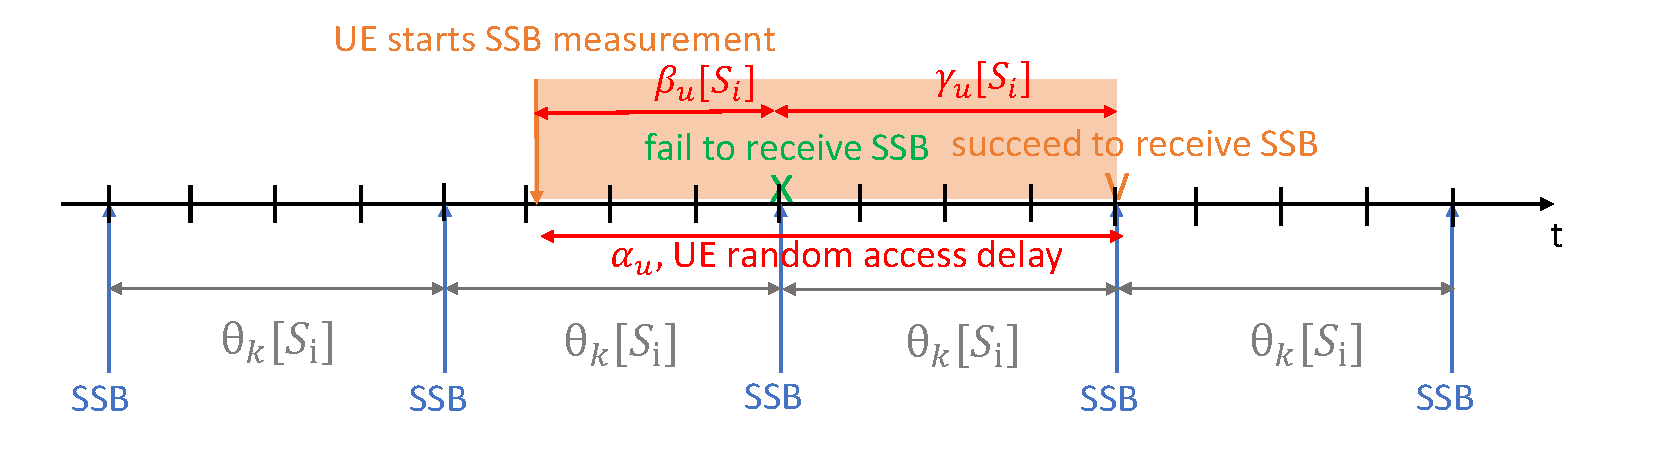
\includegraphics[width=1\textwidth]{figure/random access delay.pdf}
%     \caption{Illustration of UE random access delay. $T_u$ is decomposed into $T_u^i$ (initial waiting time) and $T_u^l$ (additional delay due to failed attempts).}
%     \label{RAD}
% \end{figure}

\section{Problem Formulation}
This section formulates the optimization problem based on recent 3GPP standardization discussions. In the 3GPP RAN1 \#116 meeting~\cite{ran1-116}, further specifications for the LEO satellite communication scenario were defined. The main challenge is to provide random access to a large number of cells with limited satellite power. Extending the SSB periodicity for some cells reduces satellite power consumption but increases UE random access delay. The transmitted SSB power also affects the success probability of the random access procedure. The trade-off among power allocation, SSB periodicity, and UE random access delay is modeled as follows:

\begin{equation}
\begin{aligned}
    & \underset{P_m[t], T_k^{SSB}[s]}{\text{min}} \sum_{u \in \mathcal{U}} \sum_{s \in \mathcal{S}} T_u[s] \\
    & \text{subject to} \\
    & \quad \sum_{m} P_{m}[t] \leq P^{total}, \quad \forall t \in \mathcal{T} \\
    & \quad P_{m}[t] \geq 0, \quad \forall m \in \mathcal{M}, t \in \mathcal{T} \\
    & \quad T_k^{SSB}[s] \leq N, \quad \forall k \in \mathcal{K}, \forall s \in \mathcal{S} \\
    & \quad T_k^{SSB}[s] \in \mathbb{N}^+, \quad \forall k \in \mathcal{K}, \forall s \in \mathcal{S} \\
\end{aligned}
\end{equation}
where $\mathbb{N}^+$ is the set with all positive integers. 

% \section{List of Symbols}
% \begin{tabular}{ll}
% \hline
% \multicolumn{2}{l}{\textbf{Symbol}} \\
% \hline
% $N$ & Number of satellites \\
% $M$ & Number of beams per satellite \\
% $K$ & Number of cells on the ground \\
% $U$ & Number of user equipments (UEs) \\
% $L_{n,k}$ & Free space path loss from satellite $n$ to cell $k$ \\
% $h_{n,k}$ & Channel gain between satellite $n$ and cell $k$ \\
% $G(\theta_{n,m,u})$ & Antenna gain for user $u$ \\
% $T^{SSB}_k$ & SSB periodicity of cell $k$ \\
% $T_u$ & Random access delay of UE $u$ \\
% $P_{n,m}$ & Transmitted power of satellite $n$'s $m$-th beam \\
% $P_s$ & Maximum transmitted power for each satellite \\
% $P_{th}$ & SSB reception threshold \\
% $Q_u$ & Number of failed SSB attempts for UE $u$ \\
% \end{tabular}